\documentclass[border=5mm]{standalone}
\usepackage{tikz}
\usetikzlibrary{shapes.geometric, arrows.meta, positioning, fit, backgrounds}

\tikzset{
    process/.style={rectangle, minimum width=3cm, minimum height=1cm, text centered, draw=black, fill=white, thick},
    arrow/.style={-Stealth, thick},
    label/.style={font=\small}
}

\begin{document}
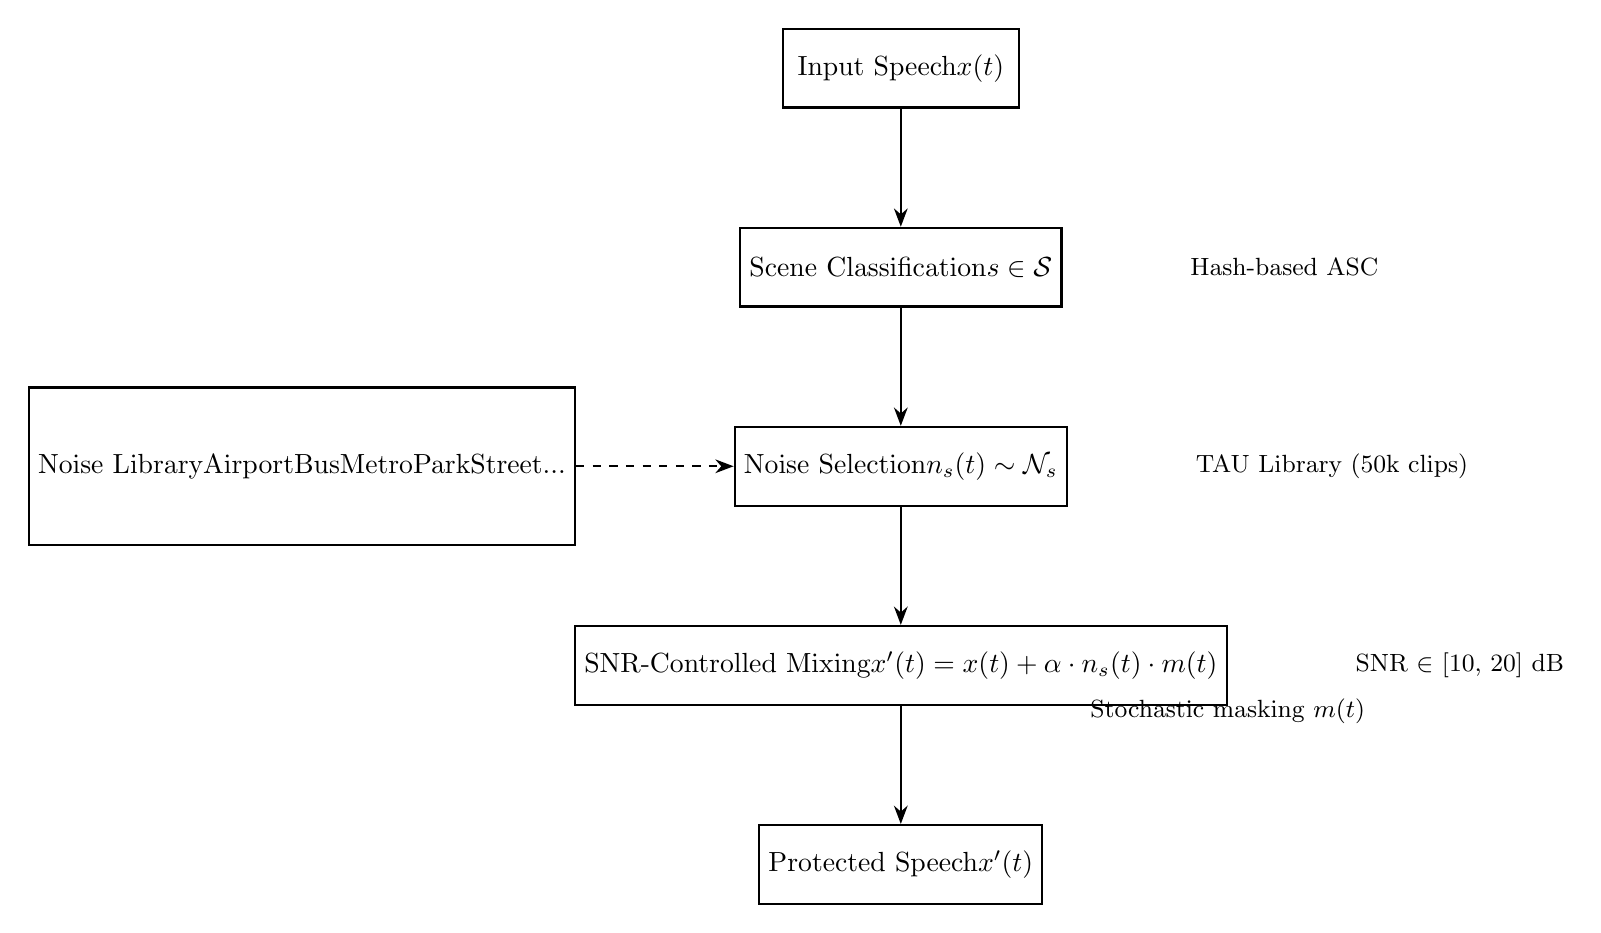
\begin{tikzpicture}[node distance=1.5cm]

% Nodes
\node (input) [process] {Input Speech\\$x(t)$};

\node (asc) [process, below=of input] {Scene Classification\\$s \in \mathcal{S}$};

\node (noise) [process, below=of asc] {Noise Selection\\$n_s(t) \sim \mathcal{N}_s$};

\node (mixing) [process, below=of noise] {SNR-Controlled Mixing\\$x'(t) = x(t) + \alpha \cdot n_s(t) \cdot m(t)$};

\node (output) [process, below=of mixing] {Protected Speech\\$x'(t)$};

% Arrows
\draw [arrow] (input) -- (asc);
\draw [arrow] (asc) -- (noise);
\draw [arrow] (noise) -- (mixing);
\draw [arrow] (mixing) -- (output);

% Side annotations
\node [label, right=1.5cm of asc] {Hash-based ASC};
\node [label, right=1.5cm of noise] {TAU Library (50k clips)};
\node [label, right=1.5cm of mixing] {SNR $\in$ [10, 20] dB};
\node [label, right=1.5cm of mixing, below=0.3cm] {Stochastic masking $m(t)$};

% Side box for noise library
\node [process, left=2cm of noise, minimum height=2cm] (lib) {Noise Library\\\\Airport\\Bus\\Metro\\Park\\Street\\...};

\draw [arrow, dashed] (lib) -- (noise);

\end{tikzpicture}
\end{document}

